\documentclass[12pt,a4paper]{report}
\usepackage[margin=1in]{geometry}
\usepackage{graphicx}
\usepackage[hidelinks]{hyperref}
\usepackage{fancyhdr}
\usepackage{array}
\usepackage{multirow}
\usepackage{booktabs}
\usepackage{listings}
\usepackage{xcolor}
\usepackage{float}
\usepackage{longtable}

% Set headheight for fancyhdr
\setlength{\headheight}{15pt}

% Header and footer
\pagestyle{fancy}
\fancyhf{}
\rhead{M.I.A: Metropolitan Information Agent}
\lhead{Project Report}
\cfoot{\thepage}

% Code listing configuration
\lstset{
    basicstyle=\ttfamily\small,
    breaklines=true,
    frame=single,
    backgroundcolor=\color{white},
    keywordstyle=\color{blue},
    commentstyle=\color{gray},
    stringstyle=\color{red},
}

% Reduce spacing
\usepackage{setspace}
\setstretch{0.95}
\usepackage{titlesec}
\titlespacing*{\chapter}{0pt}{-20pt}{10pt}
\titlespacing*{\section}{0pt}{8pt}{5pt}
\titlespacing*{\subsection}{0pt}{6pt}{3pt}

% Title configuration
\title{
    \Huge \textbf{M.I.A} \\
    \Large Metropolitan Information Agent \\
    \vspace{0.8cm}
    \large Comprehensive Project Report \\
    \vspace{0.3cm}
    \normalsize AI-Powered University Management System \\
    \vspace{1.5cm}
    \small Metropolitan University of Tirana
}
\author{
    \normalsize Development Team: Xhoi Ikonomi, Ajna Nushi, Aida Bedaj, Parashqevi Klimi, Loric Hagard \\
    \vspace{1cm}
    \small Advanced Software Engineering Project
}
\date{\small June 2026}

\begin{document}

% Title Page
\maketitle
\thispagestyle{empty}

% Table of Contents
\tableofcontents

\setcounter{page}{1}

% ============================================================================
\chapter{Executive Summary}
% ============================================================================

M.I.A (Metropolitan Information Agent) represents a comprehensive, full-stack, AI-powered university management system developed for Metropolitan University of Tirana. The system consolidates fragmented academic operations into a unified platform serving three distinct user roles: Students, Professors, and Administrators.

The core vision behind M.I.A is straightforward yet transformative: eliminate friction in university operations by providing students with instant AI-powered academic guidance, giving professors one unified workspace for all course-related operations, and providing administrators complete visibility and control over institutional data.

The standout innovation is a conversational AI adviser embedded directly in the student portal, powered by Groq or Gemini APIs. This adviser provides personalized academic guidance in natural language, addressing a critical bottleneck where students currently wait 5-7 days for adviser appointments that could be resolved in seconds. Students can ask questions like "When will I graduate?" or "What courses should I take next semester?" and receive immediate, contextual recommendations based on their academic profile.

The project timeline spans three months from April to June 2026, with a five-person development team structured around two frontend developers, two backend developers, and one AI specialist. The target user base includes over 5,000 students and 300+ faculty members at Metropolitan University of Tirana.

\section{Project Overview}

This report documents the complete design, architecture, and execution strategy for the M.I.A system. It provides a comprehensive overview of how the system addresses current institutional challenges, the technical approach taken to solve these problems, the team structure managing the project, and the criteria by which success will be measured.

The scope of this report extends from high-level vision and problem analysis through detailed system architecture, feature specifications for all three user roles, technical implementation details, project timeline and milestones, risk management strategies, and success criteria with measurable evaluation metrics.

This document is intended for multiple audiences: Metropolitan University of Tirana stakeholders and decision-makers who need to understand what the system will do and why; the development team and technical staff who need to understand how it will be built; project investors and sponsors who need to understand the scope and timeline; course instructors and academic advisers who may contribute feedback; and future maintainers and contributors who will need to understand the system design.

% ============================================================================
\chapter{Problem Statement}
% ============================================================================

Metropolitan University of Tirana currently operates academic management through a collection of disconnected systems, manual processes, and paper-based workflows that create significant friction for all stakeholders. This fragmentation has measurable negative impacts on efficiency, data quality, student experience, and institutional scalability.

\section{Current Situation and Pain Points}

\subsection{Student Experience}

Students at Metropolitan University face significant obstacles in accessing and managing their academic information. Without self-service access to academic progress, a student seeking to know their current GPA or understand their graduation timeline must submit a request to the registrar office and wait 24-48 hours for a response. Assignment submission is scattered across multiple platforms and relies heavily on email, making it easy for submissions to be lost or overlooked. There is no unified academic dashboard, forcing students to piece together information about their courses, grades, attendance records, and materials from multiple disconnected sources.

More fundamentally, students lack real-time guidance on academic planning. Booking an appointment with an academic adviser currently requires waiting 5-7 days, and if the student has questions during that waiting period or needs quick clarification on course requirements, there is no way to get assistance. No system exists to recommend courses based on a student's progress, major requirements, and graduation timeline. The only option is waiting for a human adviser to become available.

The financial aspect of student experience is equally opaque. Students have no visibility into their tuition balance, payment deadlines, or payment history. This creates confusion and prevents students from proactively managing their financial obligations.

\subsection{Professor Workflow}

Professors must juggle multiple disconnected systems to manage their courses. Grades might be tracked in spreadsheets, attendance in paper roll calls or separate files, course materials scattered across Moodle, email, and personal drives, and assignments managed through various channels. Recording grades for a single class can take 30+ minutes due to manual data entry without validation or consistency checking.

Course roster management requires coordination with the registrar office for any enrollment adjustments. There is limited visibility into student progress until final exams, making it difficult to identify and support at-risk students early. Attendance tracking is tedious, relying on manual roll calls or spreadsheet maintenance with no central visibility. Providing feedback on student work is fragmented, with no organized system for storing and communicating grades and comments back to students.

The lack of integration between these systems means professors must manually synchronize information across platforms, introducing opportunities for errors and inconsistencies.

\subsection{Administrative Operations}

The registrar office and administrative staff operate without a unified system for user management, forcing them to manage student and professor accounts separately. Report generation is primarily manual, pulling data from disconnected databases and spreadsheets. Financial operations including tuition, payments, and scholarships are managed separately from the academic system, creating data silos that prevent comprehensive institutional analysis.

Audit trails are weak, making it difficult to track who changed what data and when, creating compliance risk for accreditation and institutional reporting. Enrollment management is manual and error-prone, with no automated workflows for common operations like adding or removing students from courses. As enrollment grows, these manual processes require proportional increases in administrative staff, making the system unable to scale efficiently.

\section{Quantified Impact}

The current situation has measurable negative impacts. The registrar office spends 40-50\% of available time on manual data entry and report generation. Data inconsistencies across systems create errors in student records that require manual reconciliation. Students wait days for information they should be able to access instantly, creating frustration and preventing timely academic decisions. The system cannot grow without proportional increases in administrative staffing, limiting scalability and driving operational costs.

These problems are not rare edge cases but daily occurrences affecting the entire student and faculty population.

% ============================================================================
\chapter{Solution Overview}
% ============================================================================

M.I.A addresses these systemic challenges by consolidating all academic operations into a unified, modern, web-based platform. Rather than requiring users to navigate multiple disconnected systems, all stakeholders access a single source of truth tailored to their role and responsibilities.

\section{Core Value Proposition}

\subsection{For Students}

The M.I.A student portal transforms the academic experience from fragmented and reactive to unified and proactive. Students can view their complete academic profile in real time: current grades and GPA, attendance records by course, transcript for download, and clear progress toward graduation. Rather than waiting days for adviser appointments, students can open M.I.A and ask academic questions in natural language. "What courses should I take next semester to graduate on time?" receives an immediate, personalized recommendation based on the student's major, completed credits, GPA, and graduation requirements.

The system maintains memory of student preferences across conversations. If a student mentions they prefer morning classes and are interested in artificial intelligence, M.I.A remembers this context and incorporates it into future recommendations. Assignment submission is organized and tracked with clear status visibility. Financial information is transparent, showing tuition balance, payment schedule, and transaction history.

All of this is available 24/7, unlike human advisers. A student can get guidance at midnight before an early class, not just during office hours.

\subsection{For Professors}

Professors gain a unified workspace replacing the current collection of disconnected tools. My Courses shows all current courses with their details. A single Grades interface handles both individual grade entry and bulk uploads for an entire class. Attendance is tracked and organized by course session. Assignments are created once and viewed with all student submissions in one place. Course materials are organized and easily shared with students.

Beyond consolidation, the system provides visibility. Grade distribution histograms show the professor how the class performed on assignments. Attendance patterns highlight students missing multiple sessions. A course roster shows all enrolled students with their current grades and attendance record, enabling early identification of at-risk students who need intervention.

The administrative overhead of course management drops dramatically. What currently takes 30+ minutes to record grades for a class can be done in 5 minutes through bulk upload or streamlined individual entry with validation.

\subsection{For Administrators}

Administrators transition from manual, disconnected operations to a unified institutional view. User management is centralized: create, edit, or delete accounts and assign roles from one interface. The system overview dashboard shows key metrics: total users by role, active courses, enrollment statistics, and real-time system health.

Financial operations are integrated with academic data, enabling comprehensive reporting on fee collection, payment status, and installment compliance. Administrators can configure tuition fees per major and have those fees automatically assigned to new students. Payment tracking is transparent, showing which students have paid, which are overdue, and a complete transaction history.

Institutional reporting becomes automated rather than manual. Reports on enrollment by major, grade distribution, payment status, and course utilization can be generated on demand with accurate, current data. Audit logs track all significant operations, providing the compliance documentation needed for accreditation and institutional reporting.

% ============================================================================
\chapter{System Architecture}
% ============================================================================

M.I.A follows a modern three-tier architecture with an additional AI integration tier for the conversational adviser. This separation of concerns enables parallel development, independent scaling, and clear responsibility boundaries.

\section{Architecture Overview}

The presentation tier consists of React applications compiled and deployed as static assets. The frontend communicates exclusively through REST APIs, making the system architecture clean and decoupled. The application tier is implemented in FastAPI and Python, handling request validation, business logic, authentication, and database operations. The data tier uses PostgreSQL as the relational database and Supabase Storage for file assets like course materials and assignment submissions. The AI tier integrates with Groq or Gemini APIs for LLM inference powering the M.I.A conversational adviser.

This architecture was chosen deliberately after comprehensive technology evaluation. Each component was validated through proof-of-concept implementations before the project began.

\section{Technology Rationale}

React was selected for the frontend because it provides a component-based architecture well-suited to building three distinct portals (Admin, Professor, Student) that share some UI patterns while diverging in functionality. The ecosystem is mature with excellent developer tooling and library support. TypeScript provides static type checking, catching bugs before runtime.

Vite was chosen as the build tool for its superior developer experience. Hot module reloading means developers see changes instantly without full page refreshes. The build process optimizes production bundles aggressively, keeping bundle sizes under 150KB even with comprehensive functionality.

Tailwind CSS accelerates styling work by eliminating context-switching between HTML and CSS files. Rather than naming CSS classes, developers apply utility classes directly in markup, reducing the need to maintain separate stylesheet files. The utility-first approach has proven faster for iteration than traditional custom CSS approaches.

FastAPI on the Python backend provides excellent performance for an async runtime environment, auto-generates OpenAPI documentation directly from code, and has strong typing support through Pydantic models. These characteristics make FastAPI unusually productive for backend API development, particularly when integrating with Python-based AI libraries.

PostgreSQL is a reliable, ACID-compliant relational database well-suited to structured academic data with complex relationships. Supabase provides managed PostgreSQL hosting, eliminating operational overhead. Rather than maintaining our own database infrastructure, we leverage Supabase's expertise in hosting, backups, monitoring, and scaling.

The Groq API provides sub-100 millisecond inference latency with GPT-quality models, enabling the real-time response times necessary for a chat interface to feel responsive. Gemini is kept as a fallback option, providing redundancy and allowing cost comparison during operation.

All technologies were validated through working proof-of-concept implementations during the research phase. FastAPI was proven to handle async I/O efficiently. Groq latency was measured at <200ms, well below the 500ms target. React + Vite bundle sizes came in at <150KB, exceeding performance targets. This validation eliminated the largest technical risks before development began.

\section{Data Model}

The system's data model reflects the academic domain with tables for Users (base entity for all roles), Students (profile and progress tracking), Professors (department and title), Courses (with professor assignment), Enrollments (student-course relationships), Grades (with component structure), Attendance (session-level tracking), Assignments (course work), Submissions (student work), Chat Sessions and Messages (conversation history), and Student Preferences (M.I.A context).

Foreign key relationships enforce referential integrity. Constraints ensure data validity (grades between 0-100, weights sum appropriately, etc.). Indexes on frequently queried columns (student_id, course_id, semester) ensure query performance at scale.

% ============================================================================
\chapter{Features and Capabilities}
% ============================================================================

The M.I.A system delivers comprehensive academic management functionality across three user roles. The MVP (Minimum Viable Product) focuses on core operations that address the most pressing pain points identified during requirements analysis.

\section{Student Portal}

Students access a comprehensive academic dashboard showing their current semester at a glance. Enrolled courses appear with professor names and course materials. Current grades and GPA display prominently. Upcoming assignments show due dates. This provides an instant overview without requiring navigation to multiple screens.

The Grades section displays grades by course and semester with GPA calculation. Students see grade components (midterm, final, assignment) and understand how grades are weighted. This transparency enables students to understand their standing and identify areas for improvement.

The Courses section shows full course details: syllabus, learning outcomes, professor information, and course materials organized by topic. Students download materials directly from the portal rather than through email or external links.

Assignment management is centralized. Students see all assignments with status (assigned, submitted, graded). Submission is straightforward: upload a file or enter text directly. Once submitted, students see their submission status and any feedback provided by the professor.

The Transcript section provides a downloadable official academic transcript showing all completed courses, grades, and cumulative GPA. This is particularly valuable for job applications, graduate school applications, and other scenarios where official academic records are required.

The M.I.A Chat feature is exclusive to the student portal. Students open a chat interface and ask academic questions in natural language. M.I.A retrieves the student's academic profile (grades, completed courses, major, graduation requirements) and generates personalized, contextual responses. The system maintains conversation history and student preferences, remembering that a student prefers morning classes or is interested in specific subject areas. This enables M.I.A to provide increasingly personalized recommendations over time.

The Tuition section shows financial information: current balance, payment schedule, which installments are paid and which are pending, transaction history, and payment due dates. This transparency helps students manage their financial obligations proactively.

\section{Professor Portal}

The Professor Dashboard consolidates course management into one interface. My Courses lists all courses assigned to the professor with enrollment counts, meeting times, and quick access to course operations.

The Grades section enables efficient grade recording. Professors can enter grades individually with validation ensuring values are between 0-100 and correctly weighted. Alternatively, they can upload a spreadsheet of grades, with the system validating and importing them in bulk. This flexibility accommodates different professor preferences and significantly reduces the time spent on grade entry.

Attendance tracking is organized by course and date. Professors record who was present, absent, or late at each session. The system calculates hours present for the semester and generates attendance reports.

Assignments are created with title, description, due date, and optional file attachment. Students see assignments and submit responses through the student portal. Professors view all submissions in one place, provide grades and feedback, and mark assignments as graded.

Course Materials are uploaded once and organized by topic. Students access materials directly from the course page. This replaces the current approach of sharing materials through email or Moodle.

The Roster shows all enrolled students with quick access to individual student records. Professors see student grades and attendance patterns for their course, enabling early identification of struggling students.

\section{Administrator Portal}

The Admin Dashboard provides institutional overview. Key metrics display: total students and faculty, active courses, total enrollments, system uptime, and recent activity. This snapshot enables quick assessment of institutional status.

User Management enables creation and editing of student and professor accounts. Administrators can bulk import users from CSV files, streamlining enrollment of new cohorts. Role assignment ensures each user has appropriate access (student, professor, or administrator).

System Reports provide data-driven institutional insights. Enrollment reports show students by major and year. Grade reports show distribution of grades across the institution. Payment reports show collection status and identify overdue accounts. These reports support planning, budgeting, and compliance documentation.

Tuition Configuration enables administrators to define fees per major and academic program. Once configured, fees are automatically assigned to new students based on their major. Payment plans are configured once (e.g., three monthly installments) and automatically applied to students.

Payment Tracking shows all payments received, from which students, when, and what amount. This enables accurate financial reporting and helps identify students with financial holds or delinquent accounts.

Audit Logs record all significant operations: who logged in when, who modified which records, what changes were made. This creates an audit trail necessary for compliance and security.

\section{Phase 2 Enhancements}

Features deferred to Phase 2 for future implementation include scholarship management system, advanced financial analytics, mobile applications for iOS and Android, direct student-professor messaging, grade appeal workflow, course evaluation surveys, and advanced analytics dashboard. These features are well-understood but not critical for MVP launch.

\section{Use Case Diagrams}

\subsection{Student Portal Use Cases}
\begin{figure}[H]
\centering
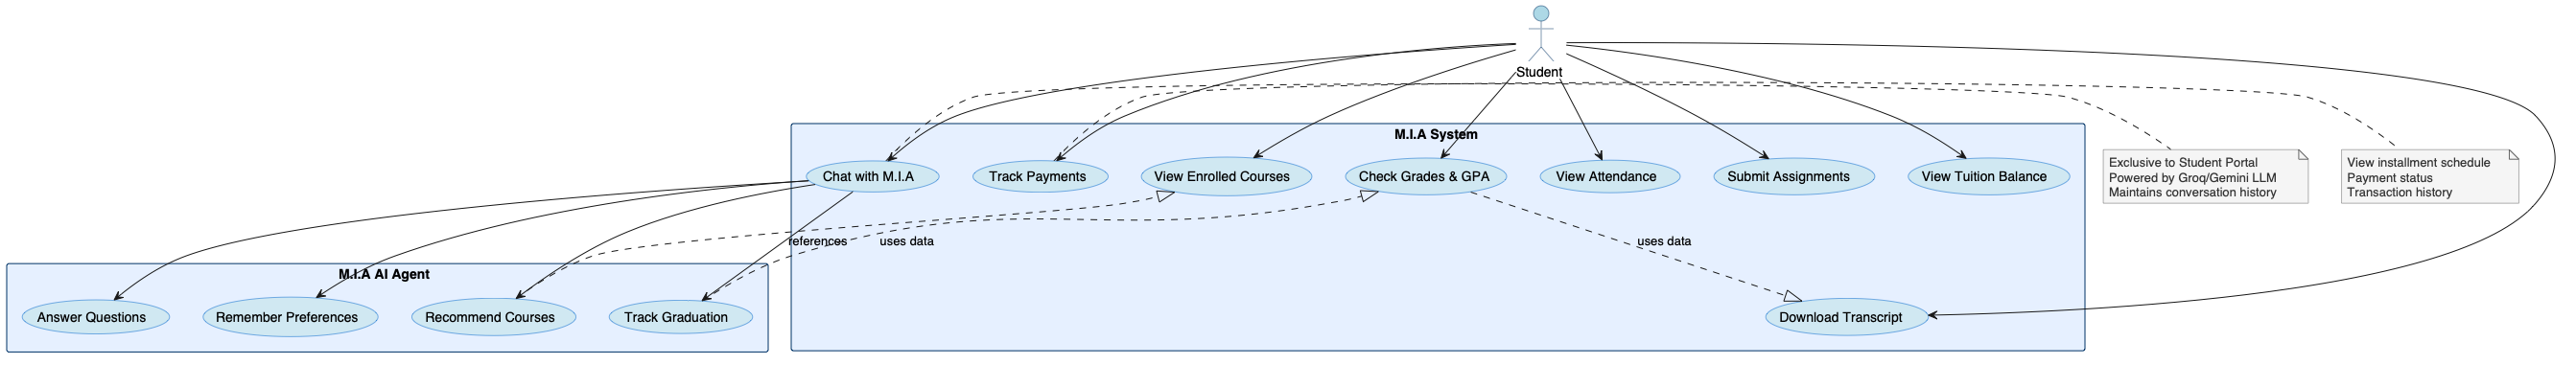
\includegraphics[width=0.95\textwidth]{use-case-student.png}
\caption{Student use cases: view grades, submit assignments, access M.I.A chat}
\end{figure}

\subsection{Professor Dashboard Use Cases}
\begin{figure}[H]
\centering
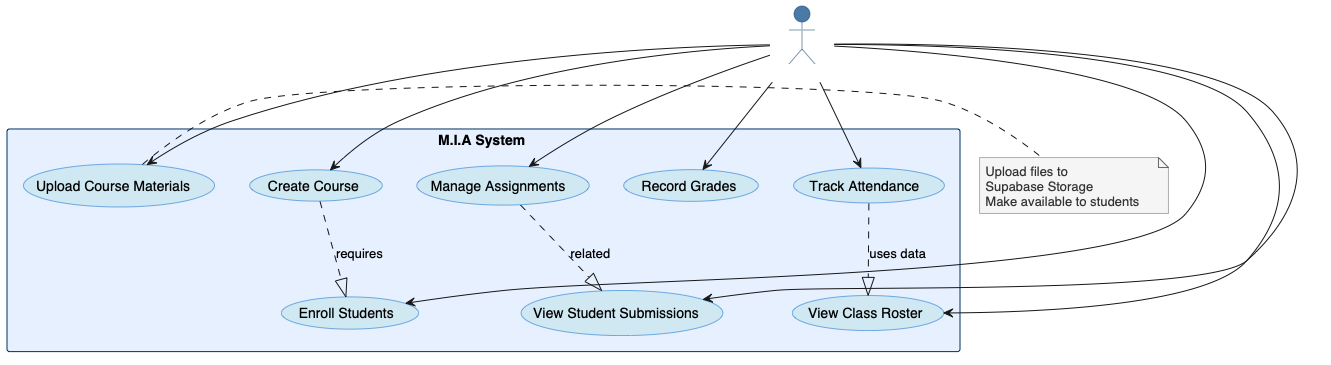
\includegraphics[width=0.95\textwidth]{use-case-professor.png}
\caption{Professor use cases: manage courses, record grades, track attendance}
\end{figure}

\subsection{Administrator Portal Use Cases}
\begin{figure}[H]
\centering
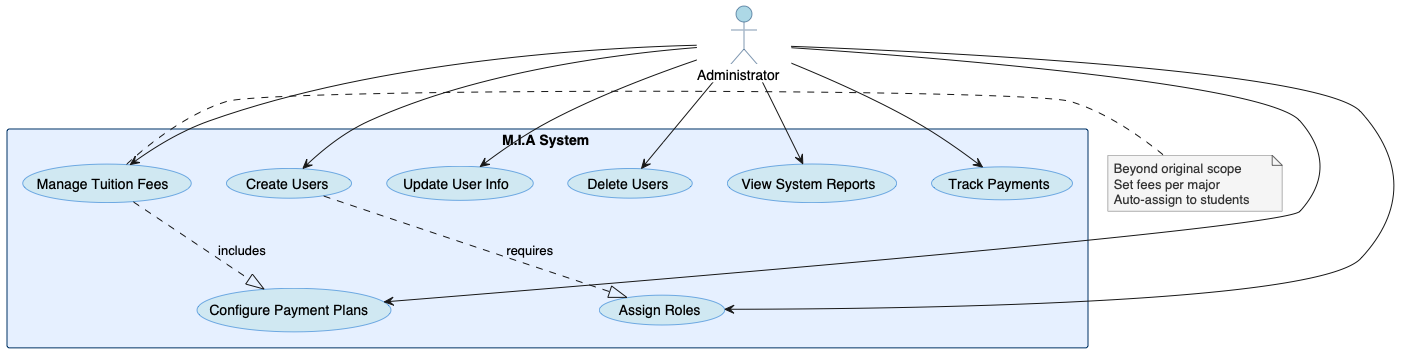
\includegraphics[width=0.95\textwidth]{use-case-admin.png}
\caption{Administrator use cases: user management, system oversight, financial operations}
\end{figure}

% ============================================================================
\chapter{Technical Implementation}
% ============================================================================

The M.I.A system is built using industry-standard technologies proven at scale. The backend REST API enforces strict validation, implements comprehensive error handling, and provides role-based access control on all protected resources. The frontend builds reusable component libraries enabling consistent UI and rapid iteration.

\section{Backend Implementation}

The backend exposes RESTful endpoints following REST conventions. Authentication uses JWT tokens, enabling stateless operation that scales horizontally. All endpoints validate input using Pydantic models, catching malformed requests before they reach business logic. Responses are consistently formatted with meaningful error messages when validation fails.

Role-based access control is implemented at the endpoint level. Every protected endpoint verifies that the authenticated user has permission to access the requested resource. A student cannot access another student's grades. A professor cannot record grades for courses they don't teach. An administrator endpoint is not accessible to students or professors.

The database is accessed exclusively through an ORM (SQLAlchemy), preventing SQL injection vulnerabilities and providing type safety. Complex queries are optimized with appropriate indexes and query analysis to ensure performance at scale.

Error handling is comprehensive. Expected errors like validation failures or permission denials return appropriate HTTP status codes with descriptive messages. Unexpected errors are logged with full stack traces for debugging while returning generic error messages to the client, preventing information disclosure.

\section{Frontend Implementation}

The React frontend is organized into reusable components, each handling a specific UI concern. A Dashboard component displays key information. A GradeTable component handles grade display and editing. These components are composed into pages: a student's Grades page includes a GradeTable, filter controls, and GPA calculation.

State management uses React hooks. useState manages local component state. useEffect handles side effects like API calls. Custom hooks abstract common patterns, reducing code duplication across components.

All API communication goes through a dedicated API client module. This centralizes error handling and request/response transformations, making it easy to add logging or retry logic globally.

Styling uses Tailwind CSS utility classes. Components are responsive by default, adapting layouts for mobile, tablet, and desktop. Dark mode is supported through Tailwind's dark mode feature, toggled at the system level.

\section{M.I.A AI Integration}

The M.I.A conversational adviser is implemented as an API endpoint that accepts user messages and returns AI-generated responses. When a student submits a chat message, the frontend sends it to the backend. The backend retrieves the student's academic profile: grades by course and semester, GPA, completed credit hours, major, graduation requirements, and stored preferences (class time preferences, interests, goals).

The backend constructs an LLM prompt that includes this context plus the student's question. This prompt is sent to the Groq or Gemini API, which returns a response within 200-500 milliseconds. The response is sent back to the frontend and displayed to the student. The message and response are stored in the database for conversation history.

Context and memory enable personalization. Student preferences stored in the database are included in prompts, allowing M.I.A to remember preferences across conversations. If a student mentions "I prefer morning classes," this is stored and included in future prompts, so M.I.A can recommend courses with morning meeting times.

\section{Process Flow Diagrams}

\subsection{M.I.A Conversational Flow}
\begin{figure}[H]
\centering
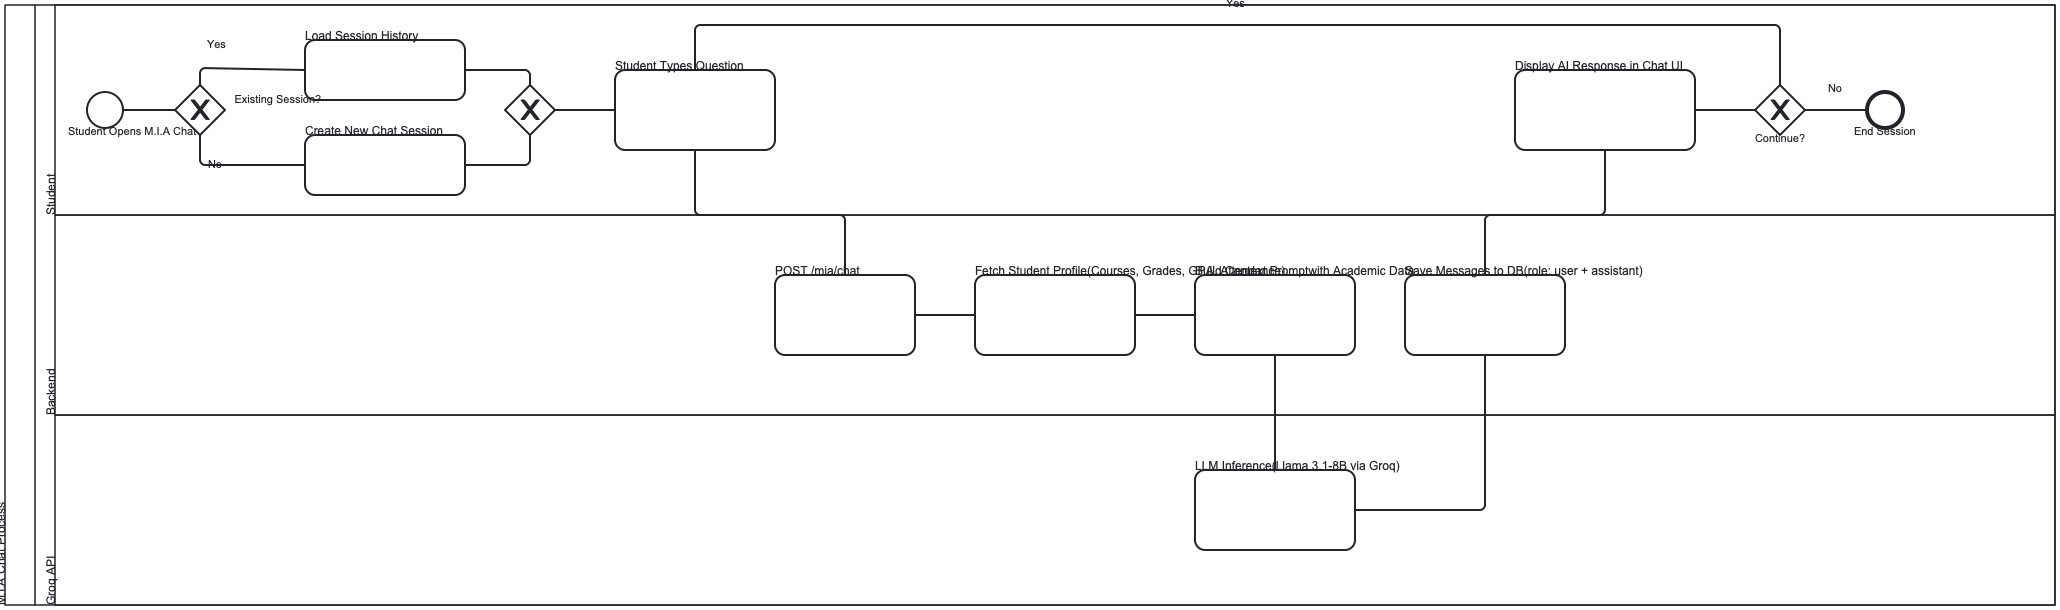
\includegraphics[width=0.95\textwidth]{M.I.A-Chat-Flow-BPMN.png}
\caption{M.I.A chat workflow: student query through LLM response and storage}
\end{figure}

\subsection{Authentication and Login Flow}
\begin{figure}[H]
\centering
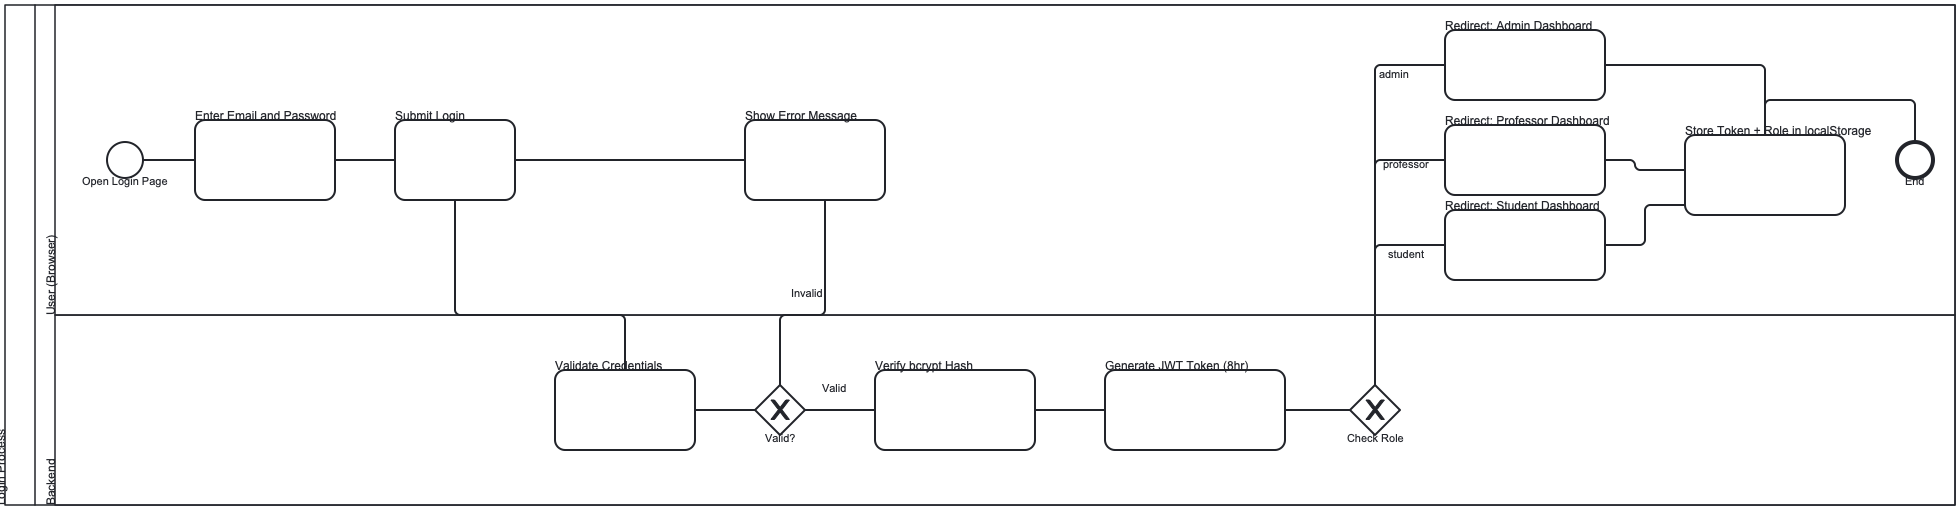
\includegraphics[width=0.95\textwidth]{Login-Flow-BPMN.png}
\caption{User login and role-based authentication and redirection}
\end{figure}

\subsection{Assignment Submission and Grading}
\begin{figure}[H]
\centering
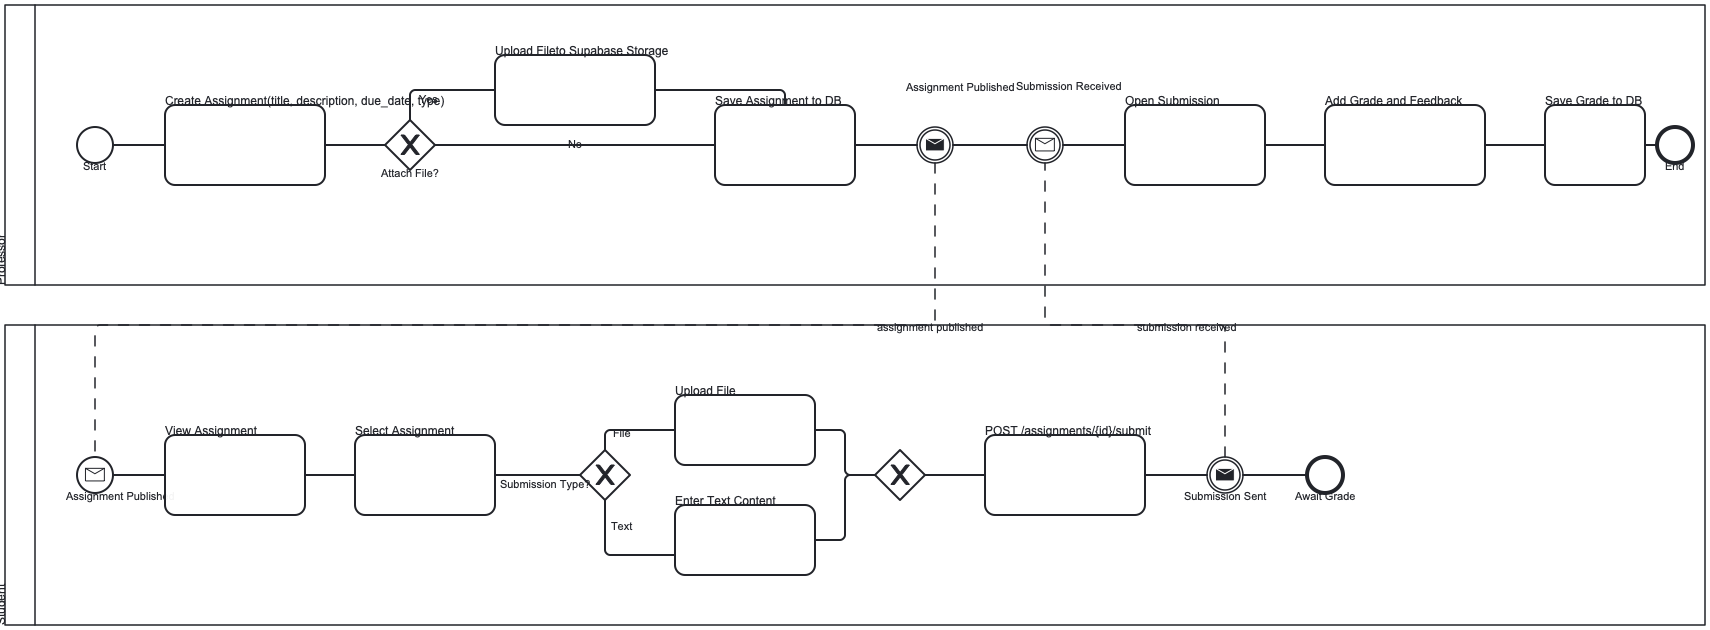
\includegraphics[width=0.95\textwidth]{Assignment-Submission-BPMN.png}
\caption{Assignment creation, student submission, and professor grading workflow}
\end{figure}

% ============================================================================
\chapter{Team and Organization}
% ============================================================================

The M.I.A development team consists of five experienced developers structured around specific domains. Xhoi Ikonomi leads frontend development and serves as project captain, responsible for overall timeline and team coordination. Ajna Nushi focuses on student-facing frontend UI including the M.I.A chat interface. Aida Bedaj implements core backend logic and database models. Parashqevi Klimi handles API routing, authentication, and Supabase integration. Loric Hagard specializes in AI integration, prompt engineering, and LLM API optimization.

This structure provides clear responsibility boundaries while enabling collaboration. Frontend developers coordinate on component design and state management. Backend developers coordinate on API contracts and database schema. All developers participate in code review to maintain quality and knowledge sharing.

The team meets weekly for status updates, feature demonstrations, blocker discussion, and sprint planning. Daily standups are asynchronous via Slack, allowing team members to catch up on progress without synchronous meetings. Code is developed on feature branches with pull request review before merging to main. All commits follow conventional commit format for clear history.

Quality standards are enforced through testing, code review, and static analysis. Unit tests provide >80\% code coverage. Pull requests require at least one team member review. TypeScript and mypy catch type errors before runtime. The codebase is formatted consistently through linters and formatters.

% ============================================================================
\chapter{Project Timeline and Milestones}
% ============================================================================

The M.I.A project spans three months from April through June 2026, structured into distinct phases. The research and validation phase runs through mid-April, where all technology choices are validated through proof-of-concept implementations. Design follows, establishing UI mockups and data models by late April. Three two-week development sprints proceed from late April through early June, with sprint 1 focusing on authentication and core API, sprint 2 on academic features, and sprint 3 on student portal and M.I.A integration.

Testing and optimization occupies the second and third weeks of June. Quality assurance testing is comprehensive, targeting zero critical bugs before launch. Documentation is finalized during this period, providing user guides and technical documentation for operations.

Final deployment preparations occur in late June. The system is deployed to the production environment and undergoes user acceptance testing with representatives from each stakeholder group. Any final issues identified during UAT are resolved before official launch.

The project culminates in late June with official go-live, when all students, professors, and administrators gain access to the system. Post-launch support for six months ensures smooth operation and provides time to gather feedback for Phase 2 planning.

% ============================================================================
\chapter{Success Criteria and Metrics}
% ============================================================================

Success for M.I.A is measured across functional, performance, adoption, and business dimensions. Functionally, all three user portals must operate reliably with zero data integrity issues. Students must be able to view grades, submit assignments, and chat with M.I.A without errors. Professors must be able to record grades and manage attendance. Administrators must be able to manage users and generate reports.

Performance targets are specific and measurable. Page load time must be under 3 seconds. API response time (95th percentile) must be under 500 milliseconds. LLM inference time must be under 2 seconds. System uptime must reach 99.5\%, meaning less than 3.5 hours of downtime per year. These targets ensure the system feels responsive and reliable.

Adoption metrics measure whether users actually embrace the system. Within 3 months of launch, target 80\% of students using the student portal at least once per week. Target 90\% of professors using the grade recording interface instead of alternative methods. Expect 100\% administrative engagement immediately. These adoption rates indicate users find the system valuable and trustworthy.

Business impact is measured through efficiency gains and user satisfaction. Target 50\% reduction in registrar office time spent on manual data entry through automation. Target 80\% of professor grade recording accomplished in 5 minutes or less through bulk upload capability. Target M.I.A satisfaction rating of 4.0 out of 5.0 from student users. Measure fee collection improvement as students gain visibility into payment obligations and can pay online.

These success criteria are specific, measurable, and achievable. They reflect the tangible improvements M.I.A brings to institutional operations and user experience.

% ============================================================================
\chapter{Risk Management}
% ============================================================================

Major risks were identified during planning and mitigation strategies established. LLM API unavailability is a potential risk: if Groq or Gemini become unavailable, M.I.A chat would not function. Mitigation includes maintaining active accounts with both providers for redundancy, implementing graceful degradation that shows helpful static responses when LLM is unavailable, and monitoring API status with alerting for immediate notification of issues.

Database performance at scale is another risk. If database queries become slow under load, the entire system would feel sluggish. Mitigation includes load testing with 5,000+ concurrent users early in development to identify bottlenecks, optimizing slow queries before launch, and implementing caching layers if needed.

Scope creep could cause schedule slippage. If requirements expand beyond the MVP, development will extend beyond the June target. Mitigation is strict scope enforcement: the captain ensures new feature requests are deferred to Phase 2, requirements are documented clearly to prevent misunderstandings, and trade-offs are made explicitly when features cannot fit in the timeline.

Data migration errors could corrupt student records during system deployment. Mitigation includes comprehensive backup strategies, validation tests that verify migrated data integrity, and a parallel run period where the old system and new system operate simultaneously, catching discrepancies before cutover.

Security vulnerabilities could expose student data. Mitigation includes security audits before launch, code review with attention to common vulnerabilities, adherence to OWASP top 10 principles, and secure credential management.

Poor M.I.A accuracy could frustrate students and reduce adoption. If M.I.A answers questions incorrectly 20\% of the time, users will lose trust. Mitigation includes beta testing with 50-100 real students before full launch, gathering detailed feedback on answer accuracy, refining prompts based on feedback, and providing human adviser contact information as fallback for critical questions.

Comprehensive risk management means these potential obstacles are anticipated and mitigation strategies are in place before issues arise.

% ============================================================================
\chapter{Client Requirements and Context}
% ============================================================================

Metropolitan University of Tirana is a leading private higher education institution in Albania serving approximately 5,000 students across five schools and 20+ academic departments. The university has motivated students and committed faculty, and modern campus facilities. However, academic operations rely on fragmented systems and manual processes that create inefficiency and prevent scaling.

The university's main objective is consolidating academic operations into a unified platform that eliminates fragmentation, enables student self-service to reduce registrar workload, and provides administrative visibility for planning and compliance. Success from the client's perspective means registrar staff time spent on manual tasks is reduced by 50\%, professors adopt the grade recording system for 90\%+ of their grading, students achieve 80\%+ adoption within three months, and the system demonstrates 99.5\% uptime reliability.

The client values modern technology that will remain relevant for 5+ years, emphasizing quality and completeness of the MVP over ambitious feature lists that would compromise delivery. They prefer managed cloud hosting (Supabase) over on-premise infrastructure, eliminating the need to maintain servers and backups internally.

Understanding client context ensures the solution aligns with institutional priorities and success metrics are relevant to actual business value.

% ============================================================================
\chapter{Conclusion}
% ============================================================================

M.I.A represents a comprehensive solution to the fragmentation and manual processes that currently characterize university academic management. By consolidating disparate systems into a unified platform with intelligent AI-powered guidance, the project directly addresses pain points affecting students, professors, and administrators daily.

The technology stack was carefully selected and validated through proof-of-concept work before development began. The architecture is modern and scalable, capable of supporting the institution's current user base and accommodating future growth. The feature set focuses on MVP completeness rather than ambitious scope, ensuring delivery by the June 2026 target.

The development team is structured for parallel work across frontend, backend, and AI components. Clear communication patterns and quality standards ensure the system will be reliable and maintainable. Comprehensive risk management identifies potential obstacles and establishes mitigation strategies before they become problems.

Success is measured through specific criteria: functional completeness, performance targets, user adoption rates, and business impact metrics. These criteria reflect both technical excellence and institutional value.

M.I.A is positioned to significantly improve the academic experience for all stakeholders at Metropolitan University of Tirana while reducing operational burden and enabling institutional scaling.

\end{document}
